% Author: Izaak Neutelings (October 2021)
% Inspiration
%   "Very special relativity - An illustrated guide", Sander Bais (2007)
%   http://people.uncw.edu/hermanr/GR/Minkowski/Minkowski.pdf
\documentclass[border=10pt,tikz]{standalone}
\usepackage{amsmath} % for \text
\usepackage{etoolbox} % ifthen
\usepackage[outline]{contour} % glow around text
\usetikzlibrary{calc} % for adding up coordinates
\usetikzlibrary{decorations.markings,decorations.pathmorphing}
\usetikzlibrary{angles,quotes} % for pic (angle labels)
\usetikzlibrary{arrows.meta} % for arrow size
\usepackage{xfp} % higher precision (16 digits?)
\contourlength{1.1pt}

\tikzset{>=latex} % for LaTeX arrow head
\colorlet{myred}{red!85!black}
\colorlet{mydarkred}{red!55!black}
\colorlet{mylightred}{red!85!black!12}
\colorlet{myfieldred}{mydarkred!5} % for S' background
\colorlet{myredhighlight}{myred!20} % highlights simultaneity in ladder paradox
\colorlet{myblue}{blue!80!black}
\colorlet{mydarkblue}{blue!50!black}
\colorlet{mylightblue}{blue!50!black!30}
\colorlet{mylightblue2}{myblue!10}
\colorlet{mygreen}{green!80!black}
\colorlet{mypurple}{blue!40!red!80!black}
\colorlet{mydarkgreen}{green!50!black}
\colorlet{mydarkpurple}{blue!40!red!50!black}
\colorlet{myorange}{orange!40!yellow!95!black}
\colorlet{mydarkorange}{orange!40!yellow!85!black}
\colorlet{mybrown}{brown!20!orange!90!black}
\colorlet{mydarkbrown}{brown!20!orange!55!black}
\colorlet{mypurplehighlight}{mydarkpurple!20} 

\begin{document}

% SPACETIME DIAGRAM - EUCLIDEAN ROTATION
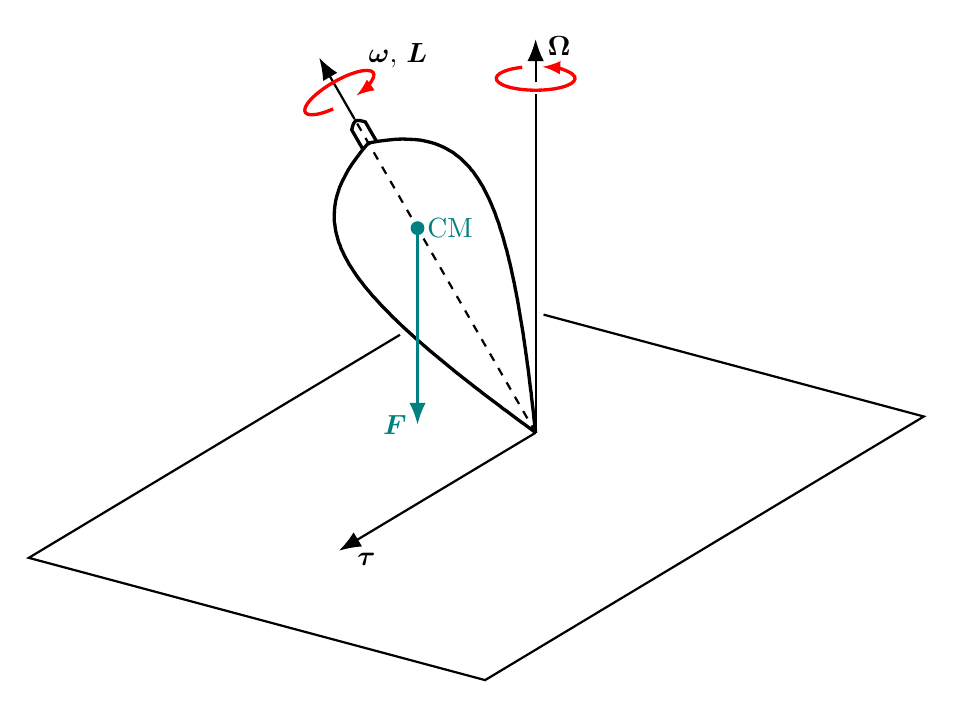
\begin{tikzpicture}[scale=5]

\begin{scope}[rotate = 30]
\draw[very thick,variable=\t,domain=0.0:1.7,samples=100] plot ({30*(sin(1.7-\t)*(1.0/(1.7-\t+0.3)-0.5))},{0.5*\t});
\draw[very thick,variable=\t,domain=0.0:1.7,samples=100] plot ({-30*(sin(1.7-\t)*(1.0/(1.7-\t+0.3)-0.5))},{0.5*\t});
\draw[very thick] (-0.02, 0.84) -- (-0.02, 0.9) 
.. controls  (0.0, 0.92) .. (0.02, 0.9) 
-- (0.02, 0.84);
\draw[thick, -{Latex[length=8pt]},] (0, 0.92) -- (0, 1.1);

\coordinate (B) at ({0.1*cos(250)}, {0.03*sin(250)+1.0});

\draw[very thick, red, ->] (B) arc [start angle=250, end angle=-70, x radius=0.1, y radius=0.03] node [above, xshift = 15pt, yshift=6pt, black] {$\boldsymbol{\omega},\, \boldsymbol{L}$};

\draw[thick, dashed] (0, 0) -- (0, 0.93);
\end{scope}

\draw[thick] (0, 0) -- (0, 0.86);
\draw[thick, -{Latex[length=8pt]},] (0, 0.89) -- (0, 1);


\draw[thick, -{Latex[length=8pt]},] (0, 0) -- (-0.5, -0.3) node [right, xshift = 3, yshift=-3] {$\boldsymbol{\tau}$};

\coordinate (A) at ({0.1*cos(110)}, {0.03*sin(110)+0.9});
\draw[very thick, red, ->] (A) arc [start angle=110, end angle=440, x radius=0.1, y radius=0.03] node [above, xshift = 6pt, black] {$\boldsymbol{\Omega}$};

\draw[thick] (0.02, 0.3) --++ (-15:1) --++ (211:1.3) --++ (165:1.2) --++ (31:1.1);

\coordinate (CM) at ({0.6*cos(120)}, {0.6*(sin(120))});
\fill[teal] (CM) circle (0.5pt) node[right] {CM};

\draw[-{Latex[length=8pt]}, teal, very thick] (CM) --++ (270:0.5) node[left] {$\boldsymbol{F}$};


\end{tikzpicture}




\end{document}